%%%%%%%%%%%%%%%%%%%%%%%%%%%%%%%%%%%%%%%%%
% Masters/Doctoral Thesis 
% LaTeX Template
% Version 1.41 (9/9/13)
%
% This template has been downloaded from:
% http://www.latextemplates.com
%
% Original authors:
% Steven Gunn 
% http://users.ecs.soton.ac.uk/srg/softwaretools/document/templates/
% and
% Sunil Patel
% http://www.sunilpatel.co.uk/thesis-template/
%
% License:
% CC BY-NC-SA 3.0 (http://creativecommons.org/licenses/by-nc-sa/3.0/)
%
% Note:
% Make sure to edit document variables in the Thesis.cls file
%
%%%%%%%%%%%%%%%%%%%%%%%%%%%%%%%%%%%%%%%%%

%----------------------------------------------------------------------------------------
%	PACKAGES AND OTHER DOCUMENT CONFIGURATIONS
%----------------------------------------------------------------------------------------

\documentclass[11pt, a4paper, oneside]{Thesis} % Paper size, default font size and one-sided paper

\graphicspath{{Pictures/}} % Specifies the directory where pictures are stored

\usepackage[square, numbers, comma, sort&compress]{natbib} % Use the natbib reference package - read up on this to edit the reference style; if you want text (e.g. Smith et al., 2012) for the in-text references (instead of numbers), remove 'numbers' 

\usepackage{minted}

\newcommand{\argmin}{\operatornamewithlimits{argmin}}
\newcommand{\argmax}{\operatornamewithlimits{argmax}}
\DeclareMathOperator{\cov}{cov}

\hypersetup{urlcolor=blue, colorlinks=true} % Colors hyperlinks in blue - change to black if annoying
\title{\ttitle} % Defines the thesis title - don't touch this

\begin{document}

\frontmatter % Use roman page numbering style (i, ii, iii, iv...) for the pre-content pages

\setstretch{1.3} % Line spacing of 1.3

% Define the page headers using the FancyHdr package and set up for one-sided printing
\fancyhead{} % Clears all page headers and footers
\rhead{\thepage} % Sets the right side header to show the page number
\lhead{} % Clears the left side page header

\pagestyle{fancy} % Finally, use the "fancy" page style to implement the FancyHdr headers

\newcommand{\HRule}{\rule{\linewidth}{0.5mm}} % New command to make the lines in the title page

% PDF meta-data
\hypersetup{pdftitle={\ttitle}}
\hypersetup{pdfsubject=\subjectname}
\hypersetup{pdfauthor=\authornames}
\hypersetup{pdfkeywords=\keywordnames}

%----------------------------------------------------------------------------------------
%	TITLE PAGE
%----------------------------------------------------------------------------------------

\begin{titlepage}
\begin{center}

\textsc{\LARGE \univname}\\[1.5cm] % University name
\textsc{\Large TDT4501 Computer Science, Specialization Project}\\[0.5cm] % Thesis type

\HRule \\[0.4cm] % Horizontal line
{\huge \bfseries \ttitle}\\[0.4cm] % Thesis title
\HRule \\[1.5cm] % Horizontal line
 
\begin{minipage}{0.4\textwidth}
\begin{flushleft} \large
\emph{Author:}\\
\authornames \\ ~ % Author name - remove the \href bracket to remove the link
\end{flushleft}
\end{minipage}
\begin{minipage}{0.4\textwidth}
\begin{flushright} \large
\emph{Supervisors:} \\
\supname % Supervisor name - remove the \href bracket to remove the link  
\end{flushright}
\end{minipage}\\[3cm]
 
% \large \textit{A thesis submitted in fulfilment of the requirements\\ for the degree of \degreename}\\[0.3cm] % University requirement text
% \textit{in the}\\[0.4cm]
% \groupname\\\deptname\\[2cm] % Research group name and department name
 
{\large \today}\\[4cm] % Date
%\includegraphics{Logo} % University/department logo - uncomment to place it
 
\vfill
\end{center}

\end{titlepage}

% %----------------------------------------------------------------------------------------
% %  DECLARATION PAGE
% %  Your institution may give you a different text to place here
% %----------------------------------------------------------------------------------------
% 
% \Declaration{
% 
% \addtocontents{toc}{\vspace{1em}} % Add a gap in the Contents, for aesthetics
% 
% I, \authornames, declare that this thesis, titled ``\ttitle'', and the work presented in it are my own. I confirm that:
% 
% \begin{itemize} 
% \item[\tiny{$\blacksquare$}] This work was done wholly or mainly while in candidature for a research degree at this University.
% \item[\tiny{$\blacksquare$}] Where any part of this thesis has previously been submitted for a degree or any other qualification at this University or any other institution, this has been clearly stated.
% \item[\tiny{$\blacksquare$}] Where I have consulted the published work of others, this is always clearly attributed.
% \item[\tiny{$\blacksquare$}] Where I have quoted from the work of others, the source is always given. With the exception of such quotations, this thesis is entirely my own work.
% \item[\tiny{$\blacksquare$}] I have acknowledged all main sources of help.
% \item[\tiny{$\blacksquare$}] Where the thesis is based on work done by myself jointly with others, I have made clear exactly what was done by others and what I have contributed myself.\\
% \end{itemize}
%  
% Signed:\\
% \rule[1em]{25em}{0.5pt} % This prints a line for the signature
%  
% Date:\\
% \rule[1em]{25em}{0.5pt} % This prints a line to write the date
% }
% 
% \clearpage % Start a new page

%----------------------------------------------------------------------------------------
%  QUOTATION PAGE
%----------------------------------------------------------------------------------------

\pagestyle{empty} % No headers or footers for the following pages

\null\vfill % Add some space to move the quote down the page a bit

\textit{\Large{``just setting up my twttr"}}

\begin{flushright}
The first Tweet ever, by Jack Dorsey on March 21, 2006
\end{flushright}

\vfill\vfill\vfill\vfill\vfill\vfill\null % Add some space at the bottom to position the quote just right

\clearpage % Start a new page

%----------------------------------------------------------------------------------------
%	ABSTRACT PAGE
%----------------------------------------------------------------------------------------

\addtotoc{Abstract} % Add the "Abstract" page entry to the Contents

\abstract{\addtocontents{toc}{\vspace{1em}} % Add a gap in the Contents, for aesthetics

Many movie recommendation systems today use collaborative filtering techniques at their core. An important challenge for collaborative filtering techniques left today is their ability to handle data sparsity. This work attempts to solve the \emph{cold start problem} by predicting movie ratings based on the perceived sentiment in Twitter search results.

The system is able to achieve a low MAE for top movies because its predictions happen to average around the average benchmark rating. It is completely unable to consistently distinguish the quality of famous top-rated movies from unknown B-films. Furthermore, it is unable to process around half of the movie titles due to a lack of Twitter search results.

}

\clearpage % Start a new page

% %----------------------------------------------------------------------------------------
% %  ACKNOWLEDGEMENTS
% %----------------------------------------------------------------------------------------
% 
\setstretch{1.3} % Reset the line-spacing to 1.3 for body text (if it has changed)

\acknowledgements{\addtocontents{toc}{\vspace{1em}} % Add a gap in the Contents, for aesthetics

I would like to thank my supervisors, Heri Ramampiaro and Helge Langseth, for lots of good advice, while at the same time allowing me a great extent of freedom in planning and executing this project.

I would also like to thank the people behind the DatumBox service, who made this project a joy to implement.

}
\clearpage % Start a new page

%----------------------------------------------------------------------------------------
%	LIST OF CONTENTS/FIGURES/TABLES PAGES
%----------------------------------------------------------------------------------------

\pagestyle{fancy} % The page style headers have been "empty" all this time, now use the "fancy" headers as defined before to bring them back

\lhead{\emph{Contents}} % Set the left side page header to "Contents"
\tableofcontents % Write out the Table of Contents

\lhead{\emph{List of Figures}} % Set the left side page header to "List of Figures"
\listoffigures % Write out the List of Figures

\lhead{\emph{List of Tables}} % Set the left side page header to "List of Tables"
\listoftables % Write out the List of Tables

%----------------------------------------------------------------------------------------
%	ABBREVIATIONS
%----------------------------------------------------------------------------------------

\clearpage % Start a new page

\setstretch{1.5} % Set the line spacing to 1.5, this makes the following tables easier to read

\lhead{\emph{Abbreviations}} % Set the left side page header to "Abbreviations"
\listofsymbols{ll} % Include a list of Abbreviations (a table of two columns)
{
\textbf{MAE} & \textbf{M}ean \textbf{A}verage \textbf{E}rror \\
\textbf{RMSE} & \textbf{R}oot \textbf{M}ean \textbf{S}quare \textbf{E}rror \\
\textbf{SaaS} & \textbf{S}oftware \textbf{a}s \textbf{a} \textbf{S}ervice \\
\textbf{SVM} & \textbf{S}upport \textbf{V}ector \textbf{M}achine \\
}

%----------------------------------------------------------------------------------------
%  PHYSICAL CONSTANTS/OTHER DEFINITIONS
%----------------------------------------------------------------------------------------
% 
% \clearpage % Start a new page
% 
% \lhead{\emph{Glossary}} % Set the left side page header to "Physical Constants"
% 
% \listofwords{ll} % Include a list of Physical Constants (a four column table)
% {
% \textbf{Tweet}    & A Twitter message \\
% \textbf{DatumBox} & A machine learning SaaS \\
% }

% %----------------------------------------------------------------------------------------
% %  SYMBOLS
% %----------------------------------------------------------------------------------------
% 
% \clearpage % Start a new page
% 
% \lhead{\emph{Symbols}} % Set the left side page header to "Symbols"
% 
% \listofnomenclature{lll} % Include a list of Symbols (a three column table)
% {
% $a$ & distance & m \\
% $P$ & power & W (Js$^{-1}$) \\
% % Symbol & Name & Unit \\
% 
% & & \\ % Gap to separate the Roman symbols from the Greek
% 
% $\omega$ & angular frequency & rads$^{-1}$ \\
% % Symbol & Name & Unit \\
% }

% %----------------------------------------------------------------------------------------
% %  DEDICATION
% %----------------------------------------------------------------------------------------
% 
% \setstretch{1.3} % Return the line spacing back to 1.3
% 
% \pagestyle{empty} % Page style needs to be empty for this page
% 
% \dedicatory{For/Dedicated to/To my\ldots} % Dedication text
% 
% \addtocontents{toc}{\vspace{2em}} % Add a gap in the Contents, for aesthetics

%----------------------------------------------------------------------------------------
%	THESIS CONTENT - CHAPTERS
%----------------------------------------------------------------------------------------

\mainmatter % Begin numeric (1,2,3...) page numbering

\pagestyle{fancy} % Return the page headers back to the "fancy" style

% Include the chapters of the thesis as separate files from the Chapters folder
% Uncomment the lines as you write the chapters

% Chapter 1

\chapter{Introduction} % Main chapter title

\label{Chapter1} % For referencing the chapter elsewhere, use \ref{Chapter1} 

\lhead{Chapter 1. \emph{Introduction}} % This is for the header on each page - perhaps a shortened title

%----------------------------------------------------------------------------------------

% \emph{Context; motivation for the project; problem statement; outline of dissertation.}

\section{Motivation}

% Movie recommendations have come a long way, but still they seem to be lacking in a few ways.
% 
% Most services supplying automated recommendations
% \begin{enumerate}
%   \item don't provide the context and background for each recommendation
%   \item don't consider public opinion and hype
% \end{enumerate}

Many movie recommendation systems today use collaborative filtering techniques at their core. Although collaborative filtering has many advantages that have let it attain its position as one of the dominant algorithms in the field, there are still quite a few weaknesses left to remedy. Among others, two important challenges for collaborative filtering techniques left today are 1) their ability to handle data sparsity~\cite{Su:2009:SCF:1592474.1722966}, and 2) their ability to explain predictions~\cite{Herlocker:2000:ECF:358916.358995}.

I will take a somewhat untraditional approach in an attempt to mitigate these issues: can data mined from one of today's largest sources of user-generated content, Twitter, contribute enough relevant information to solve both the problem of data sparsity and result explanation?

\subsection{Data sparsity in collaborative filtering}

The data sparsity problem has several sides to it~\cite{Su:2009:SCF:1592474.1722966}.

Here, we will take a closer look at the \emph{cold start} problem -- or more specifically: the \emph{new item problem}. It occurs when a new item enters the system and there is no rating history to base similarity measures on, leaving a barebones collaborative filtering algorithm without anything to base predictions on -- until, of course, some users rate it. If this is the case for a large number of items, we say that we have poor \emph{coverage}.

Second, 

\subsection{Twitter}

Twitter is one of the largest sources of user-generated content available today. It launched in 2006, was incorporated in 2007, and has seen active user growth ever since. At the time of writing, Twitter has more than 230 million registered users sending around 500 million Tweets per day.\footnote{Numbers from \url{https://about.twitter.com/company}.}

One of the most interesting things about Twitter is its simplicity. Each message is limited to 140 characters in length, for no other apparent reason than to force its author to formulate messages very concisely, as well as significantly lower the threshold for publishing content compared to traditional blogging services~\cite{Java:2007:WWT:1348549.1348556}.

Furthermore, 76\% of Twitter's active users are on mobile -- enabling use of the service from anywhere. Combined with Twitter's well-established REST API, this provides us with a robust source of real-time data on almost any subject.

I'll delve further into aspects of using Twitter as a data source in section~\ref{sec:twitter_data}.

% ----------------------------------------------------------------------------------------------------------------------

% Recommendation systems, as seen in commercial products in 2013, seldom provide any context to go with its recommended products other than statements like ``Because you watched X you might like Y.''
% 
% Netflix, the movie subscription service, quite recently began suggesting movies based on what your Facebook friends had watched -- thereby taking a solid step in the direction of social recommendations.
% These suggestions, however, have one underlying assumption that may not always apply:
% what the displayed friend has watched is relevant to your choice of content.
% 
% Furthermore, the social components in most contemporary recommendation systems are \emph{personal}.
% This approach has some clear advantages in that it uses \emph{your} social network as a basis for suggesting content, but there are also some downsides to this:
% 
% \begin{itemize}
%   \item They don't take \emph{novelty} into consideration.
%   \item They don't take \emph{hype} into consideration.
%   \item They leverage only a microscopic portion of the available opinions on content that is available in social media.
% \end{itemize}
% 
% These personal suggestions seems to be a trend in contemporary approaches to social recommendations.
% We'll have a look at something a bit different.

% \subsubsection{A different approach to social media recommendations}

%----------------------------------------------------------------------------------------

\section{Research Questions}

\emph{@REWORK}

In this thesis, I'll mostly examine \emph{improving a set of recommendations} taking social media data into account, and not so much try to generate new recommendations in their own right -- although I might make a go of it if the data should prove agreeable.

I will rather look at ways of using copious\footnote{\emph{Copious} in the sense that the size of the data source is arbitrarily large.}, unpersonal\footnote{\emph{Unpersonal} in the sense that the data is not related to a single hypothetical user of the system.} social media data to \emph{filter} sets of recommendations.

More specifically, the aim is to find answers to the following questions:

\begin{enumerate}
  \item Can sentiment analysis of large quantities of unpersonal social media data be used to effectively filter or provide context to recommendations?
  \item Can unpersonal social media data in any way generate reliable ratings of its own?
  \item How do we evaluate our efforts in order to answer the above questions?
\end{enumerate}

%----------------------------------------------------------------------------------------

\section{Overview and Summary}

This paper is organized as follows.
Chapter~\ref{Chapter2} surveys relevant literature, similar applications, and provides an in-depth analysis of Twitter data and the Twitter API.
Chapter~\ref{Chapter3} 

%----------------------------------------------------------------------------------------

% Chapter 2

\chapter{Survey} % Main chapter title

\label{Chapter2} % For referencing the chapter elsewhere, use \ref{Chapter1} 

\lhead{Chapter 2. \emph{Survey}} % This is for the header on each page - perhaps a shortened title

%----------------------------------------------------------------------------------------

% \emph{Review of relevant literature; review of similar software products or tools.}

\section{Similar applications} % (fold)
\label{sec:similar_applications}

Some people have attempted the same task as in this thesis, though with another type of social data. Singh et al. \cite{Singh2011} investigated a ``formulation, where [they] combined the content-based approach with a sentiment analysis task to improve the recommendation results.'' Their approach is very similar to our approach, but differs in two important ways:

\begin{enumerate}
  \item It uses user reviews from IMDB as content source\footnote{IMDB does not provide open API access at the time of writing.}, and not a more general source of sentiment-carrying content -- as in our case, with Twitter.
  \item It is generates recommendations based on genre input.
\end{enumerate}

% section similar_applications (end)

%----------------------------------------------------------------------------------------

\section{Twitter data} % (fold)
\label{sec:twitter_data}

Micro-blogging services such as Twitter have enormous amounts of data on almost every topic imaginable. Content is limited in length, and users react to each others' content by ``re-tweeting'', ``favoriting'' or ``replying to'' it. This leaves us with a source of textual data that is:

\begin{description}
  \item[Instant] Users express reactions to events as they experience them.
  \item[Weighted] Users weigh each others' content by interacting with it.
  \item[Concise] Due to limitations on content length, users must express themselves concisely.
\end{description}

Now, for a look at the ways in which we are able to access this data.

\subsection{Relevant parts of the Twitter API} % (fold)
\label{sub:relevant_parts_of_the_twitter_api}

The various endpoints in the Twitter REST API is divided into 16 categories, spanning everything from search and user timelines to suggested users to follow and spam reporting. A full overview of the available API endpoints is available on Twitter's REST API pages\footnote{\url{https://dev.twitter.com/docs/api/1.1}}.

Of these, only two categories are of relevance, namely \emph{Search} and \emph{OAuth}.

OAuth is only relevant because it enables us to search, so we won't elaborate further on how we use it.

\subsubsection{The Twitter search API}
\label{ssec:search_api}

The Twitter search API\footnote{\url{https://dev.twitter.com/docs/api/1.1/get/search/tweets}} is a JSON-based REST API, and it takes the following notable parameters:

\begin{description}
  \item[\texttt{q}] \hfill \\
    A UTF-8, URL-encoded search query of 1,000 characters maximum, including operators.
  \item[\texttt{result\_type}] \hfill \\
    Specifies what type of search results you would prefer to receive.
\end{description}

In addition, there are parameters to control the number of messages returned, language, date ranges etc.

The \texttt{q} parameter, the search query, is obviously of great importance, as it is the one we primarily will be using to target our search.

The \texttt{q} parameter supports a wide range of operators.\footnote{The full list is available here: \url{https://dev.twitter.com/docs/using-search}} It supports the typical boolean operators (AND, OR, and NOT), as well as specifying exact search phrases, but it also supports more domain-specific operators:

\begin{description}
  \item[From/to/referencing user] \hfill \\
    Only return messages from or to a specific user, or simply mentioning a specific user somewhere in its message.
  \item[Date ranges] \hfill \\
    Support for ``since'' and ``until'' constraints.
  \item[Other] \hfill \\
    Support for things like only returning messages with links, messages submitted via a specific client type, and messages asking a question.
\end{description}

All operators can be combined, and the regular space serves as an AND clause in this regard.

In addition to the aforementioned operators, the API supports returning tweets matching either a positive or negative sentiment -- a feature which should seem very relevant to the task at hand. However, no information was seemingly available on the mechanics behind it, and after some manual testing it was concluded that it also lacked quite severely in its precision.

The other parameter central to our application is the \texttt{result\_type}. It allows us to switch between three possible heuristics for which results that are returned from the search. We have the choice between three valid values: \texttt{recent}, \texttt{popular}, or \texttt{mixed} tweets -- the latter being a combination of the first two, and also the default.

To know which one to choose, we need to know what constitutes a popular tweet.

\subsubsection{What constitutes a popular Tweet?}

On Twitter, there are several ways of interacting with the system. Terms like ``follow'', ``mention'', ``favorite'', and ``retweet'' are all more or less domain-specific to Twitter, so before moving on -- let's break them down.

\begin{description}
  \item[Follow] \hfill \\
    Users consume each others' content by following each other. The number of followers users have range from 0 to more than 40 million. Following is a one-way relationship, and there is often a big difference in the number of users \emph{following} and \emph{being followed by} a user.
  \item[Reply] \hfill \\
    Users can mention each other in tweets by prepending a username with ``@''. This same mechanism is used to reply to others' content. When replying, the content the Tweet was replying to is stored along with the reply, forming a conversation tree.
  \item[Favorite] \hfill \\
    Users can favorite content, which notifies the content owner and boosts the content in search results etc. It is also trivial to extract all content a particular user has favorited.
  \item[Retweet] \hfill \\
    When a user chooses to retweet another user's content, that content is ``forwarded'' to the user's followers.
\end{description}

One of the greatest benefits of Twitter as a data source is that all these interactions are completely transparent\footnote{Users can make their own content ``private'', but their interactions with other users' non-private content are nonetheless public.}, and can thus be used freely when querying for popular content.

% subsection relevant_parts_of_the_twitter_api (end)

\subsection{Novelty of available data} % (fold)
\label{sub:novelty_of_available_data}

As briefly mentioned, part of the hypothesis is that Twitter data is usable for predicting ratings for new content, where collaborative filtering systems perform worse than otherwise.

Novelty, however, is an inherently fundamental quality of Twitter data, even as a data source.
The Twitter search API simply does not expose data more than about a week old.
As it is put in their search API guidelines as of December 2013~\cite{UsingTwitterSearchAPI}, ``The Search API is not complete index of all Tweets, but instead an index of recent Tweets. At the moment that index includes between 6-9 days of Tweets.''

This quality makes Twitter data less than useful when it comes to predicting ratings for movies old enough to have calmed in public debate -- a category which, not surprisingly, includes the vast majority of available movies.

% subsection novelty_of_available_data (end)

\subsection{Twitter as a Data Source} % (fold)
\label{sub:twitter_as_a_data_source}

There are vast opportunities in managing to understand a data source with the qualities discussed above, but alas -- the diversity and free nature of Twitter as a publishing platform comes at a price: \emph{there is a lot of noise}.
That is not to say that there is little relevant information, but when the service is designed to have such a low threshold for contributing content, a low signal-to-noise ratio seems inevitable.
We will return to the issue of noise in chapter~\ref{sec:evaluation_metrics}, where we try to evaluate correlations between movie titles in our test data and Tweets about the same titles.

This problem of finding content carrying relevant information turns out to perhaps be the biggest challenge of the entire study.

% subsection twitter_as_a_data_source (end)

% section twitter_data (end)

\section{The sentiment classifier} % (fold)
\label{sec:the_sentiment_classifier}

Much has already been written on the topic of sentiment analysis of Twitter data~\cite{go2009twitter, go2009twitterdistant, pak2010twitter, agarwal2011sentiment, kouloumpis2011twitter}. This paper, however, is not about improving or analyzing these methods and techniques. What is required is a technique that is good enough to \emph{indicate} the sentiment of \emph{a set of messages}.

For sentiment analysis, I have therefore selected the Twitter sentiment classifier provided by DatumBox, a machine learning SaaS. They provide a broad suite of services within many fields of machine learning. See figure~\ref{fig:datumbox_api} for an overview of their current functionality within the document classification category\footnote{The complete list is currently available at \url{http://www.datumbox.com/api-sandbox/}.}.

\begin{figure}[h]
  \centering
    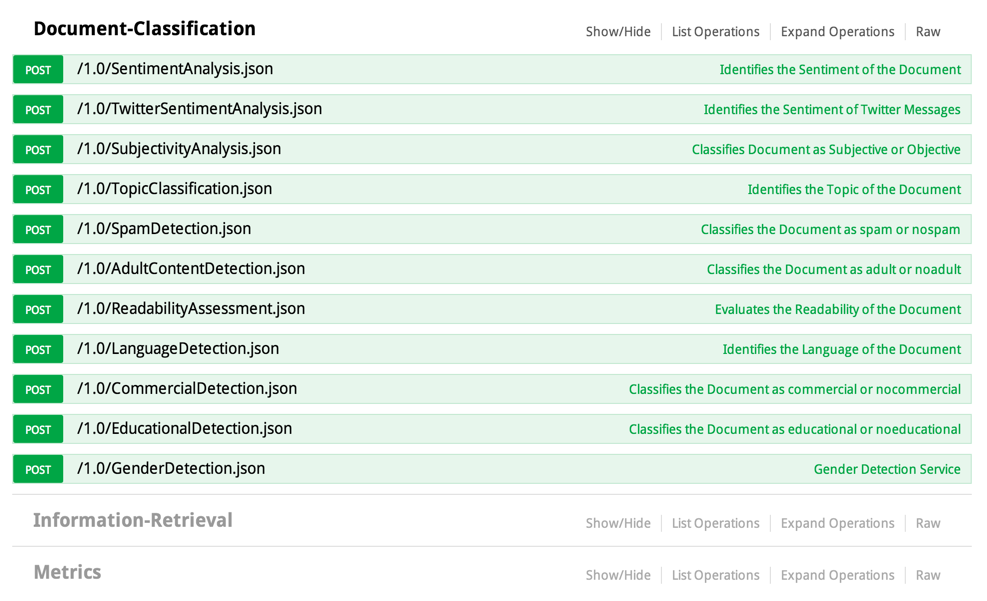
\includegraphics[width=\textwidth]{Figures/datumbox_api}
  \caption{The current endpoints in the DatumBox API in the category ``Document Classification''.}
  \label{fig:datumbox_api}
\end{figure}

Naive Bayes classifiers in general, as well as details regarding the DatumBox implementation, are described in section~\ref{sec:sentiment_analysis_impl}.

\subsection{Alternative approaches}

Two of the most relevant alternatives to the Naive Bayes, SVM and Max Entropy, are also perfectly capable of performing sentiment classification. This section will describe them briefly, with emphasis on how they perform the sentiment classification task. This is well described in the literature~\cite{pang2002thumbs}, so this survey will not go into great detail.

Max Entropy has been shown to perform several text classification tasks often better than the Naive Bayes, but it also sometimes performs worse~\cite{Nigam99usingmaximum}. The underlying principle of maximum entropy is that without further knowledge, uniform distributions should always be preferred. Training data lay constraints on the distribution, and let us know where the most uniform solutions are.

A Support Vector Machine (SVM) is a large-margin classifier, as opposed to both Naive Bayes and Max Entropy's probabilistic approaches. For a typical two-category case, classifying documents as either positive or negative, SVM attempts to find a hyperplane represented by a vector $\vec{\sigma}$ which not only separates the document vectors $\vec{d}$ of one class from the other, but which also maximizes this margin.

Since none of these approaches are particularly dominant in the literature, the simplest solution -- the Naive Bayes classifier provided to us through the DatumBox API -- was chosen.

\section{The Netflix rating dataset}
\label{sec:netflix_dataset}

For evaluating the results, the Netflix rating dataset was used as a benchmark.

The accompanying Readme file descibes the dataset in the following way:

\begin{quote}
  The movie rating files contain over 100 million ratings from 480 thousand
  randomly-chosen, anonymous Netflix customers over 17 thousand movie titles.  The
  data were collected between October, 1998 and December, 2005 and reflect the
  distribution of all ratings received during this period.  The ratings are on a
  scale from 1 to 5 (integral) stars.
\end{quote}

The data used in this work consists of two different types of files.

First, an overview of available movies is available in CSV format, with lines containing the following fields:

\begin{enumerate}
  \item Movie ID
  \item Year of release
  \item Movie title
\end{enumerate}

In a separate directory, 17770 files named by their associated movie ID contain lines of individual ratings, with the following attributes:

\begin{enumerate}
  \item Customer ID
  \item Rating
  \item Date
\end{enumerate}

Unfortunately, the Netflix rating dataset is no longer publicly available, allegedly due to a lawsuit regarding privacy concerns\footnote{\url{http://www.wired.com/threatlevel/2009/12/netflix-privacy-lawsuit/}}.

For more details on how the data was used to evaluate results, please see chapter~\ref{Chapter5}.
 
% Chapter 3

\chapter{Requirements} % Main chapter title

\label{Chapter3} % For referencing the chapter elsewhere, use \ref{Chapter1} 

\lhead{Chapter 3. \emph{Requirements}} % This is for the header on each page - perhaps a shortened title

% \emph{How requirements were captured; discussion of major requirements (referring to Appendix A for details).}
% 
% \emph{Forklar hvordan du satt opp kravene.}
% 
% \emph{Men ikke ha med en fullstendig oversikt over kravene her!}

Although the methods described in this paper aims to be as agnostic as possible with regards to what type of sentiment carrying input is used, we have selected the microblogging service Twitter -- and the available Twitter data has some specific qualities we'll try to make use of to improve the quality of our results.

\section{Relevant Qualities of Twitter Data} % (fold)
\label{sec:relevant_qualities_of_twitter_data}

As previously mentioned, ``Tweets'' can be \emph{favorited}, \emph{retweeted}, and \emph{replied to}.
Additionally, we can tell how big reach an author has by counting the number of \emph{followers} he/she has, and use this as another indication of content popularity.

We want to be able to use the data as a source of implicit ratings. To be able to, we need to quantify the significance of these verbs.
Oard~and~Kim~\cite{Oard98implicitfeedback,Oard01modelinginformation} and Kelly~and~Teevan~\cite{Kelly03implicitfeedback} have developed a framework for classification of online (@TODO)...
We adapt it to the domain of Twitter data, and wind up with table~\ref{tab:behavior_class}.

\begin{table}[h]
  \begin{center}
    \begin{tabular}{|llcl|}
      \hline
      \textbf{Original} & \textbf{Ours} & & \textbf{Action} \\
      \hline
      Create    & Create   & $\rightarrow$ & Tweet \\
      \hline
      Examine   & Consume  & $\rightarrow$ & Follow \\
      \hline
      Annotate  & Evaluate & $\rightarrow$ & Reply \\
      \hline
      Retain    & Endorse  & $\rightarrow$ & Favorite \\
      \hline
      Reference & Forward  & $\rightarrow$ & Retweet \\
      \hline
    \end{tabular}
  \end{center}
  \caption{Classification of microblogging behavior}
  \label{tab:behavior_class}
\end{table}

To clarify the classifications of table~\ref{tab:behavior_class}, let's break the terms down.

\begin{description}
  \item[Tweet]
    A user posts content to Twitter, in the form of a new post.
    A Tweet can have a maximum of 140 characters.
    Due to the size restrictions, tweets often contain links to websites.
  \item[Follow]
    Users consume each others' content by following each other.
    The number of followers users have range from 0 to more than 40 million.
    Following is a one-way relationship, and there is often a big difference in the number of users following and being followed by a user.
  \item[Reply]
    Users can mention each other in tweets by prepending a username with ``@''.
    This same mechanism is used to reply to others' content.
    When replying, the content the Tweet was replying to is stored along with the reply, forming a conversation tree.
  \item[Favorite]
    Users can favorite content, which notifies the content owner and boosts the content in search results etc.
    It is also trivial to extract all content a particular user has favorited.
  \item[Retweet]
    When a user chooses to retweet content, that content is ``forwarded'' to the user's followers, and boosts the content in search results etc.
\end{description}

% section relevant_qualities_of_twitter_data (end)


% Chapter 4

\chapter{Design} % Main chapter title

\label{Chapter4} % For referencing the chapter elsewhere, use \ref{Chapter1} 

\lhead{Chapter 4. \emph{Design}} % This is for the header on each page - perhaps a shortened title

%----------------------------------------------------------------------------------------

% \emph{How the product was designed, with discussion of design alternatives (referring to Appendix B for details).}
% 
% \emph{Diskuter de viktigste funksjonene i ditt design og hvordan det har utviklet seg, fremhev noen nye/originale funksjoner.}
% 
% \emph{Ikke ha med design dokumentasjon her!}

The basic architecture in figure~\ref{fig:1_basic_architecture} reflects this. Our work will be aimed at the component labelled \emph{A}.

\begin{figure}[h]
  \centering
    \begin{verbatim}
       -------------------                       --------------------------
      |                   |         ---         |                          |
      |  Recommendations  | -----> | A | -----> |  Better Recommendations  |
      |                   |         ---         |                          |
       -------------------           ^           --------------------------
                                     |
                                     |
                               ------------
                             /              \
                            |  Social Media  |
                             \              /
                               ------------
    \end{verbatim}
  \caption{The basic architecture of a system described in this thesis. We mainly describe the component labelled \emph{A}.}
  \label{fig:1_basic_architecture}
\end{figure}

%----------------------------------------------------------------------------------------

% Chapter 5

\chapter{Evaluation} % Main chapter title

\label{Chapter5}

\lhead{Chapter 5. \emph{Evaluation}} % This is for the header on each page - perhaps a shortened title

%----------------------------------------------------------------------------------------

% \emph{Beskriv hvordan du vurderer arbeidet ditt. Oppsummer evalueringsresultatene, og bruk dem til å vurdere ditt eget arbeid kritisk. Vær ærlig om eventuelle mangler. Hva betyr resultatene?}

\begin{itemize}
  \item When rating popular and well-known movies\footnote{The sample in question consisted of ``Pulp Fiction'', ``The Shining'', ``Mission: Impossible'', ``The Matrix'', ``The Godfather'', ``Forrest Gump'', and ``A Clockwork Orange''.} the predicted ratings achieve a correlational coefficient of 0.75 with regard to average Netflix ratings for the same movie.
  \item B-movies or older less-known movies rarely collect enough Twitter search results to warrant any further analysis.
  \item Movies with titles that are fairly common words or expressions in their own right achieve very low precision, and often return only noise. This is hard to detect without manual interference. Need to perform some sort of Named Entity Disambiguation, maybe something like the techniques outlined in Cucerzan~\cite{NamedEntityDisambiguationWiki} or Sarmento~\cite{NamedEntityDisambiguationWS} (is elaboration needed?).
\end{itemize}

\section{Evaluation metrics} % (fold)
\label{sec:evaluation_metrics}

To find out how the Twitter-based predictions fare, we will simply use the average of the available Netflix ratings of the same titles as benchmark ratings.

To compute error, the MAE (Mean Average Error) metric will be used. With predictions $p$ and benchmark ratings $r$, we will compute the MAE of $N$ sample movies in the following way:

\begin{equation}
  \text{MAE} = \frac{1}{N} \sum_{i=1}^N |p_i - r_i|
  \label{eq:mae}
\end{equation}

As a baseline metric, the MAE of the average of all the benchmark ratings is used:

\begin{align}
  \text{MAE}_\text{baseline} = \sqrt{ \frac{1}{N} \sum_{i=1}^N (\bar{r} - r_i)^2 }
\end{align}

To measure the correlation between predictions and ratings, Pearson's $r$ is used. It is calculated in the following way:

\begin{equation}
  \rho_{X,Y} = \frac{\cov(X, Y)}{\sigma_X \sigma_Y}
\end{equation}

\subsection{Why MAE?} % (fold)
\label{sub:why_mae}

Two error metrics were considered for evaluating the system: MAE and RMSE. We specifically consider MAE because of its simplicity, and RMSE because of its widespread use in the domain of evaluating movie recommendation algorithms\footnote{It was the only error metric targeted by the Netflix Prize, whence the Netflix training data originate.}.

First, let's have a look at RMSE. It is calculated in the following manner for $N$ predictions $p$ and benchmark ratings $r$:

\begin{equation}
  \text{RMSE} = \sqrt{ \frac{1}{N} \sum_{i=1}^N (p_i - r_i)^2 }
\end{equation}

The main downside to RMSE is that it is complex. It varies with three different qualities of the errors, namely

\begin{enumerate}
  \item the variability within the distribution of error magnitudes
  \item the square root of the number of errors
  \item the average error magnitude (MAE)
\end{enumerate}

The MAE, on the other hand -- as defined in~\eqref{eq:mae} -- is a lot simpler.

The goal for the evaluation of this application is to enable us to reason over the applicability of the general approach taken, not to objectively compare this specific application to other competing systems. For this, the simplicity and clarity of MAE is prioritized over RMSE's expressiveness, and will serve as the main error metric.

\section{Comparison of results from different movie types} % (fold)
\label{sec:comparison_of_results_from_different_movie_types}

Let us have a look at two sample runs. The first one selects a sample of 10 random movies from the entire set of movies in the test set, while the second run is restricted to movies present in IMDB's top 250 list (as described in section~\ref{sec:evaluation_impl}).

The results shown below are consistent with the magnitude of those gathered from evaluating other corresponding samples.

Both runs were performed with the same system parameters, apart from the top movie constraint in the second run, the most important ones listed in table~\ref{tab:run_parameters}.

\begin{table}[h]
  \begin{center}
    \begin{tabular}{ll}
      \textbf{Max. document count} & At most 25 Twitter documents were analyzed per title. \\
      \textbf{Threshold}           & 5 Twitter messages required to start sentiment analysis. \\
      \textbf{Result type}         & ``Mixed'' \\
    \end{tabular}
  \end{center}
  \caption{Parameters for evaluated test runs.}
  \label{tab:run_parameters}
\end{table}

\subsection{Run 1: Sample drawn from entire test set}

\begin{table}[h]
  \begin{center}
    \begin{tabular}{|l|rr|r|}
      \hline
      \textbf{Title} & \textbf{Prediction} & \textbf{Variance} & \textbf{Benchmark} \\
      \hline
      Chill Out          & 4.28 & 1.37 & 2.49 \\
      First Kid          & 4.48 & 1.21 & 3.59 \\
      Paparazzi          & 3.75 & 1.39 & 3.39 \\
      That Thing You Do! & 4.80 & 0.60 & 3.53 \\
      Undercover Brother & 4.05 & 1.59 & 3.10 \\
      The Backyard       & 4.47 & 1.36 & 2.36 \\
      Black Cat          & 3.80 & 1.70 & 2.30 \\
      Dangerous Game     & 3.83 & 1.52 & 2.54 \\
      So Little Time     & 3.60 & 1.80 & 3.10 \\
      Play for Me        & 2.60 & 1.96 & 2.42 \\
      \hline
    \end{tabular}
  \end{center}
  \caption{Test run for a sample of movies randomly selected from the entire test set.}
  \label{tab:test_run_all}
\end{table}

This run gives a MAE of 1.08, and a correlational coefficient of 0.39. However, these numbers vary greatly between each run. Subsequent runs with other randomly sampled movies yield the following:

\begin{enumerate}
  \item MAE: 1.16, correlational coefficient: 0.16
  \item MAE: 0.62, correlational coefficient: -0.56
  \item MAE: 0.84, correlational coefficient: -0.11
\end{enumerate}

Specifically, it is worth noting that the predictions in general grossly overshoot the benchmarks, which becomes especially clear in the comparative line plot in figure~\ref{fig:predictions_benchmark_rand}.

For the first run, it is worth pointing out that 7 movie titles were discarded for not meeting the required threshold of 5 Twitter search results. On average, approximately 50\% of the titles are discarded on this criteria.

\begin{figure}[h]
  \centering
    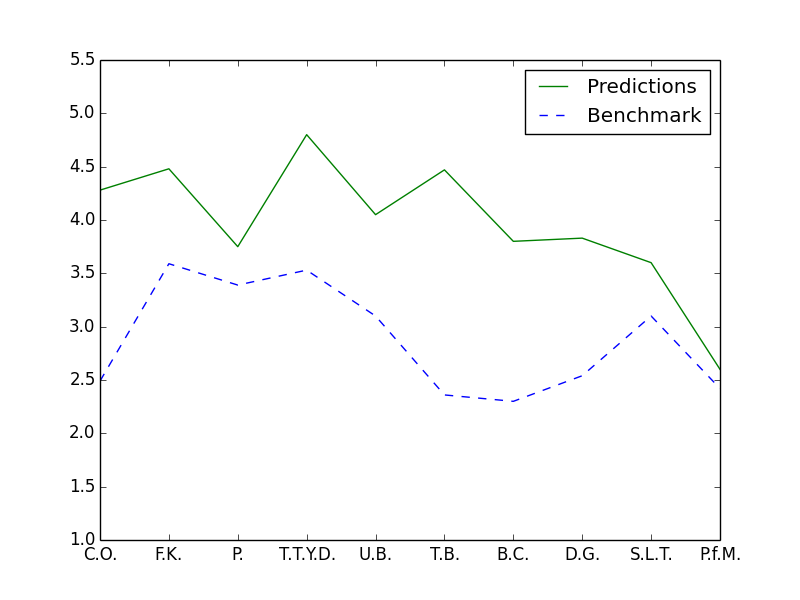
\includegraphics[width=.8\textwidth]{Figures/plots/predictions_benchmark_rand}
  \caption{Run 1: Line plot of predictions vs. benchmark value.}
  \label{fig:predictions_benchmark_rand}
\end{figure}

\subsubsection{Noisy Twitter search results}

Most of the Twitter results listed in table~\ref{tab:test_run_all} were in fact not about the movie in question. In fact, \emph{all} the search results that were evaluated on behalf of the first movie, ``Chill Out'', were about watching other movies, only mentioning ``chill out'' in the same message more or less at random.

The same is the case for several other movies in the listed sample run.

\subsection{Run 2: Sample drawn from IMDB's top 250 list}

\begin{table}[h]
  \begin{center}
    \begin{tabular}{|l|rr|r|}
      \hline
      \textbf{Title} & \textbf{Prediction} & \textbf{Variance} & \textbf{Benchmark} \\
      \hline
      The Kid             & 3.96 & 1.57 & 3.32 \\
      Metropolis          & 3.48 & 1.17 & 3.40 \\
      Reservoir Dogs      & 4.28 & 1.11 & 4.00 \\
      The Usual Suspects  & 4.04 & 1.51 & 4.37 \\
      Monsters, Inc.      & 3.64 & 1.76 & 4.28 \\
      A Beautiful Mind    & 4.44 & 1.33 & 3.97 \\
      Requiem for a Dream & 3.08 & 2.00 & 3.79 \\
      Million Dollar Baby & 4.20 & 1.60 & 4.16 \\
      City of God         & 4.76 & 0.11 & 4.10 \\
      Jurassic Park       & 3.80 & 1.60 & 3.80 \\
      \hline
    \end{tabular}
  \end{center}
  \caption{Test run for a sample of movies randomly selected from IMDB's top 250 list.}
  \label{tab:test_run_popular}
\end{table}

This run gives a MAE of 0.38, and a correlational coefficient of 0.40.

Subsequent runs with the same parameters yield the following:

\begin{enumerate}
  \item MAE: 0.78, correlational coefficient: 0.16
  \item MAE: 0.58, correlational coefficient: -0.27
  \item MAE: 0.52, correlational coefficient: 0.23
\end{enumerate}

The comparative plot in figure~\ref{fig:predictions_benchmark_pop} is better adjusted with regard to overshooting the benchmark values. However, the plot fails to emphasize is that the degree of correlation is approximately the same in both runs.

\begin{figure}[h]
  \centering
    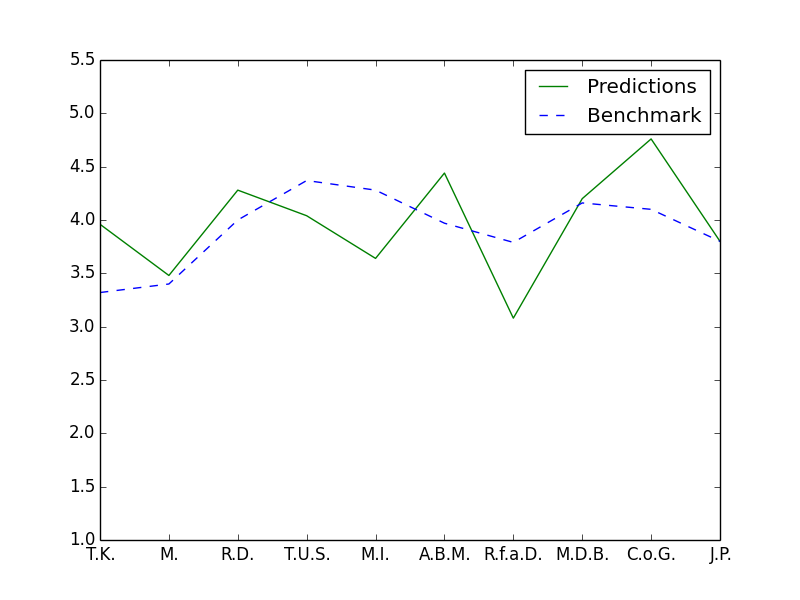
\includegraphics[width=.8\textwidth]{Figures/plots/predictions_benchmark_pop}
  \caption{Run 2: Line plot of predictions vs. benchmark value.}
  \label{fig:predictions_benchmark_pop}
\end{figure}

\subsection{Evaluation result comparison} % (fold)
\label{sub:evaluation_result_comparison}

Up to this point, the predictions have only been compared with the benchmarks. Here, they will be compared to each other.

First, the benchmarks. Let the set of benchmark ratings for run 1 be denoted $R_1$, and similarly the benchmark ratings from run 2 $R_2$. As expected, the average benchmark ratings from run 2 -- the top movies -- are clearly above the ones from run 1.

\begin{align}
  \bar{R}_1 = 2.882 \\
  \bar{R}_2 = 3.919
\end{align}

A difference of more than $1.0$. A number along these lines is what we want to see as the difference between the average predictions from the two runs.

However, when we perform the same mean value comparison for the \emph{predictions} from the two runs, denoted $P_1$ and $P_2$, we see a different pattern:

\begin{align}
  \bar{P}_1 = 3.966 \\
  \bar{P}_2 = 3.968
\end{align}

A difference of only 0.002 -- a mere nothing.

This result repeats in approximately the same way for every run: the average rating predictions seem to be completely disassociated with the benchmark ratings of the test set.

% subsection evaluation_run_summary (end)

% Chapter 6

\chapter{Conclusion} % Main chapter title

\label{Chapter6}

\lhead{Chapter 6. \emph{Conclusion}} % This is for the header on each page - perhaps a shortened title

%----------------------------------------------------------------------------------------

% \emph{I konklusjonen din, beskriv status for ditt arbeid. Oppsummer hva du har oppnådd, sammenlignet med hva du opprinnelig ønsket å oppnå. Relater arbeidet til tidligere relevant arbeid. Foreslår videre arbeid som du tror vil være verdt.}

I thought that the data would contain too much noise to be usable in any other way than to annotate and -- in the best of cases -- adjust ratings of content where the social sentiment disagreed strongly with the proposed rating.

However, for certain kinds of content, the predictions generated by Twitter were more or less spot on the same as the ones from Netflix, as shown in chapter~\ref{Chapter5}.

This leads me to believe that Twitter as a data source for recommendations can have a greater role than that of augmenting recommendations coming from elsewhere. (@TODO More specifically....)

Moving towards a conclusion:

\begin{enumerate}
  \item Twitter's strongest suite lies in its abundance of novel content.
  \item Some of the traditional CF systems' weakest points relate to recommending novel content.
  \item Augmenting new content, with extremely sparse user ratings, might well be a good application.
\end{enumerate}

\section{Suggestions for further work} % (fold)
\label{sec:suggestions_for_further_work}

Suggestions to further work:

\begin{itemize}
  \item Applying NED to Twitter entities.
  \item Further improving sentiment analysis of informal texts.
  \item CRF og sentimentanalyse? -- klassifisere bort tekster? filtrere i et første steg.
  \item Nyere filmer -- tråle IMDB for nye filmer.
  \item
    Gi kontekst til Netflix-ratings:
    (1. legge til adjektiver?, 2. kontrastifisere positive/negative adjektiver. ordsky?)

  \item \emph{Hva vil jeg jobbe med til våren?}
\end{itemize}

% section suggestions_for_further_work (end)


%----------------------------------------------------------------------------------------
%	THESIS CONTENT - APPENDICES
%----------------------------------------------------------------------------------------

\addtocontents{toc}{\vspace{2em}} % Add a gap in the Contents, for aesthetics

\appendix % Cue to tell LaTeX that the following 'chapters' are Appendices

% Include the appendices of the thesis as separate files from the Appendices folder
% Uncomment the lines as you write the Appendices

% Appendix A

\chapter{Requirements} % Main appendix title

\label{AppendixA} % For referencing this appendix elsewhere, use \ref{AppendixA}

\lhead{Appendix A. \emph{Requirements}} % This is for the header on each page - perhaps a shortened title


% % Appendix B

\chapter{Design Documents} % Main appendix title

\label{AppendixB} % For referencing this appendix elsewhere, use \ref{AppendixA}

\lhead{Appendix B. \emph{Design Documents}} % This is for the header on each page - perhaps a shortened title


% % Appendix C

\chapter{Evaluation Results} % Main appendix title

\label{AppendixC} % For referencing this appendix elsewhere, use \ref{AppendixC}

\lhead{Appendix C. \emph{Evaluation Results}} % This is for the header on each page - perhaps a shortened title



\addtocontents{toc}{\vspace{2em}} % Add a gap in the Contents, for aesthetics

\backmatter

%----------------------------------------------------------------------------------------
%	BIBLIOGRAPHY
%----------------------------------------------------------------------------------------

\label{Bibliography}

\lhead{\emph{Bibliography}} % Change the page header to say "Bibliography"

\bibliographystyle{unsrtnat} % Use the "unsrtnat" BibTeX style for formatting the Bibliography

\bibliography{Bibliography} % The references (bibliography) information are stored in the file named "Bibliography.bib"

\end{document}  